\documentclass[12pt]{article}
\usepackage[a4paper,top=2cm,bottom=2cm,left=2.5cm,right=2.5cm,marginparwidth=1.75cm]{geometry}
%\geometry{landscape}                % Activate for for rotated page geometry
%\usepackage[parfill]{parskip}    % Activate to begin paragraphs with an empty line rather than an indent
\usepackage{graphicx}
\usepackage{float}
\usepackage{hyperref}
\usepackage{subfigure}
\usepackage{rotating}
\usepackage{booktabs}
\usepackage{amssymb}
\usepackage{amsmath}
\usepackage{amsthm}
\usepackage{color}
\usepackage{gb4e}
\noautomath

%\usepackage[natbib=true,maxcitenames=2,bibstyle=authoryear, style=apa]{biblatex}
\usepackage{natbib}
\bibliography{interferencebib}
\usepackage{lineno,xcolor,clipboard,graphicx}


\usepackage{csquotes}
%\DeclareLanguageMapping{american}{american-apa}

\usepackage{marginnote}
\setcounter{section}{-1}

\openclipboard{output-reviews}

\renewcommand{\qedsymbol}{\rule{0.7em}{0.7em}}

\usepackage{epstopdf}
\newcommand{\revised}[1]{{\color{black}{#1}}}

\DeclareGraphicsRule{.tif}{png}{.png}{`convert #1 `dirname #1`/`basename #1 .tif`.png}

\title{Response to editor and reviewers (JML-24-17)}
\author{Pia Schoknecht, Himanshu Yadav, and Shravan Vasishth}
%\date{}                                           % Activate to display a given date or no date


\usepackage{xr}

\makeatletter
\newcommand*{\addFileDependency}[1]{% argument=file name and extension
\typeout{(#1)}% latexmk will find this if $recorder=0
% however, in that case, it will ignore #1 if it is a .aux or 
% .pdf file etc and it exists! If it doesn't exist, it will appear 
% in the list of dependents regardless)
%
% Write the following if you want it to appear in \listfiles 
% --- although not really necessary and latexmk doesn't use this
%
\@addtofilelist{#1}
%
% latexmk will find this message if #1 doesn't exist (yet)
\IfFileExists{#1}{}{\typeout{No file #1.}}
}\makeatother

\newcommand*{\myexternaldocument}[1]{%
\externaldocument{#1}%
\addFileDependency{#1.tex}%
\addFileDependency{#1.aux}%
}

\myexternaldocument{elsarticle-template-harv}

\begin{document}
\hfill \today
%\section{}
%\subsection{}

\noindent \textbf{Prof.\ Christopher Jarrold}\\
\noindent \textbf{Associate Editor}\\
\noindent \textbf{Journal of Memory and Language}
\vskip 1em

\noindent \textbf{Response letter for Submission JML-24-17, 2nd round of revisions}
\vskip 2em
\noindent Dear Prof. Jarrold, 
\vskip 1em
with my co-authors Shravan Vasishth and Himanshu Yadav, I would like to submit the second revision of our article titled ``Do syntactic and semantic similarity lead to interference effects? Evidence from self-paced reading and event-related potentials using German''.


We are grateful for the thoughtful and constructive comments and suggestions from yourself and the reviewers, and feel that the quality of the manuscript has been greatly improved by the revisions.
To address the concern that we overstate the implications of our findings, we have clarified at various places in the abstract and discussion of our results that our findings only apply to the present design. 

Clarifying text has been added in this second round of revisions (e.g., regarding the implications, the prolonged reading times starting at the distractor and the use of syntactic and semantic cues), and we have shortened the manuscript length by four pages. We have removed redundant text passages (e.g., in the description of the SPR results).

The OSF repository has bee made public to ensure general accessibility. We have updated the link in the manuscript accordingly.

Below, we separately address each comment from the reviewers and yourself. All changes have been highlighted in the revised manuscript. The actionable parts of the comments are highlighted in bold.

\vskip 1em
\noindent Sincerely,
\vskip 1em
\noindent Pia Schoknecht\\
Postdoctoral researcher\\
Department of Linguistics\\
University of Potsdam, Germany
\thispagestyle{empty}
\newpage

\section*{Editor's comments} 
\subsection*{Comment E.1}
\begin{quote}
``Dear Dr. Schoknecht,

Thank you for submitting your revised manuscript to the Journal of Memory and Language. This has now been reviewed by the same three experts who reviewed the previous submission, and you can find their comments below.

You will see from these that all three reviewers appreciate the thoroughness with which you responded to the issues raised on the initial submission. Reviewers 1 and 3 raise some remaining points but recommend acceptance, while Reviewer 2 is less persuaded that your revisions have adequately addressed their concerns. Given this set of reviews, I have come to a `revise' decision because I would like you to have one more go at addressing the remaining points made by all three reviewers.

I do not anticipate sending out the next version for review again, but rather anticipate being in a position to accept it at that point. However, it's important to note that that is not guaranteed, and one reason I have come to a `revise' rather than `accept subject to minor revisions' is that, like Reviewer 1, I was unable to access your data via your OSF link. \textbf{It is very important to us at JML that data are readily accessible, and that accessibility needs to be in place before any potential acceptance decision}.''
\end{quote}

\subsubsection*{Response to E.1}
We have made the OSF repository public to grant general accessibility. We paste our data availability statement below.

\begin{quote}
    \Paste{link}
\end{quote}



\subsection*{Comment E.2}
\begin{quote}
``The other key points I would like to ask you to pay particular attention to in any response to the current set of reviews are:

\textbf{Reviewer 2 and 3's clear view that you still overstate the implications of your findings in places}.''
\end{quote}

\subsubsection*{Response to E.2}
We have revised the manuscript to be more cautious regarding the implications and generalizability of our findings. The most that we can claim in this paper is that \textit{in the particular experiment design} that we use here, we have no decisive evidence for syntactic interference. But this does not mean that syntactic interference cannot occur in general. We make this point clear in our revision now.

See the revised abstract and related text edits below.

\bigskip
\noindent Revised abstract:

\begin{quote}
    \Paste{abstract}
\end{quote}

In the general discussion (page \pageref{gendisccaveat}), we already had an unambiguous statement 
that, given the broader evidence in sentence processing, syntax generally does play a role in dependency completion:

\begin{quote}
    \Paste{gendisccaveat}
\end{quote}

We have now made this section even more explicit by stating that syntactic interference may well play a role in some other, stronger syntactic manipulation than the one that we used, and that our own results would need to be independently replicated in order to establish their robustness:

\begin{quote}
    \Paste{gendisccaveat2}
\end{quote}



\noindent Related text edits on pages \pageref{thisdesign1}, \pageref{synsem}, \pageref{thisdesign2} and \pageref{thisdesign3}:

\begin{quote}
    \Paste{thisdesign1}
\end{quote}

\begin{quote}
    \Paste{thisdesign4}
\end{quote}

\begin{quote}
    \Paste{thisdesign2}
\end{quote}

\begin{quote}
    \Paste{thisdesign3}
\end{quote}


\subsection*{Comment E.3}
\begin{quote}
``\textbf{Reviewer 2's additional point 1 that asks whether you have changed that particular analysis}.''
\end{quote}

\subsubsection*{Response to E.3}
Yes, we changed all analyses in the first revision. As we had explained in the response to reviewers on August 29, 2024 (specifically in the response letter and our responses to the comments E.2 and R3.5), the priors were changed from directional priors in the original version to symmetrical priors in the revised version. Additionally, we changed the method with which the Bayes factors were computed. Initially, we had used bridge sampling, but in the revision, we switched to the Savage-Dickey method because only using that method we were able to compare models with random slopes (this was also explained in the previous response letter, Response to R1.7). These changes did not change the results qualitatively, but led to some numerical changes which probably piqued the reviewer's interest.


\subsection*{Comment E.4}
\begin{quote}
``and \textbf{their final point about the length of the current version of the manuscript}.''
\end{quote}

\subsubsection*{Response to E.4}
We have removed repetitions in the description of the statistical analyses and have shortened the description of the self-paced reading results (and the comparison to the previous studies). This reduced the length of the manuscript by four ages; after the first round of revisions the main text ended on page 77, now it ends on page 73. 

\section*{Reviewer \#1} 

\subsection*{Comment R1.1}
\begin{quote}
``I was the Reviewer \#1 of the previous version of the manuscript.

All my concerns are addressed in this revision, so I am happy to say I don't see reasons to ask for resubmission or for another round of major, significant revisions. I found it a solid paper in the first round already, but with the revisions and especially given the modified and extended analysis, I find the whole story more convincing and also, fair.

I do have some suggestions. In my view these are only minor. They mainly concern just the way things are presented or discussed. I list my comments by page.

p. 16: osf data etc.

I wanted to check those, but \textbf{when I clicked the link, it said I don't have permissions and that I need to request access}.''
\end{quote}

\subsubsection*{Response to R1.1}
We have made the OSF repository public to grant general accessibility (see also our Response to E.1).

\subsection*{Comment R1.2}

\begin{quote}
``p. 17, SPR experiment

\textbf{Did the analysis include any cut-off point for reading times to exclude data? I could not find this in the manuscript. If it did, could this information be included?} If not, I would strongly suggest to use this. In my own experience with Prolific, I noticed the following very common pattern: people basically do not read around 10-20\% of experimental items - that is, for quite a significant subset of participants I noticed that they have super fast reading times on some subset of items, most likely because they just rushed through those items by just pressing the space bar and keeping it pressed. This is sometimes followed by a long waiting time at some other point, so those participants would not be outliers when we check the total time in the experiment. These people and their data would not be excluded by checking their answers to comprehension questions, especially if only a small subset of items has comprehension questions, like one third, as in this experiment (basically, they could still easily pass with around 90\% success rate). So if this was not checked, it would be good to check and \textbf{consider removing RTs based on small/large cut-off points and to see whether that affects the analysis. If this was done already, it would be good to report more details, in particular, the cut-off points and also the amount of data that was removed this way}.''
\end{quote}

\subsubsection*{Response to R1.2}
We excluded reading times below 150 ms and above 3000 ms. This affected 4.9\,\% of the data. We have added this information to the manuscript on page \pageref{trim}:

\begin{quote}
    \Paste{trim}
\end{quote}

\subsection*{Comment R1.3}
\begin{quote}
``p. 36: ``Regarding the possibility that sentence structure confounds caused the effects in the pre-critical region(.)"

\textbf{I wonder whether it would make sense to briefly summarize what the sentence structure confound should be.} Otherwise the whole paragraph is hard to follow for readers who did not read or do not remember Mertzen et al. (2023).''
\end{quote}
\subsubsection*{Response to R1.3}
We have added the following text to the manuscript on page \pageref{confound} (above the sentence which was quoted by the reviewer):

\begin{quote}
    \Paste{confound}
\end{quote}


\subsection*{Comment R1.4}
\begin{quote}
``p. 51: ``For more discussion of the role of structural retrieval cues, see Franck and Wagers (2020) and Arnett and Wagers (2017)."

\textbf{It would be good to cite Kush et al. (2015) here} (after all, a significant portion of Franck and Wagers, 2020, builds on Kush et al. 2015 to explore ways to deal with structural cues).

Kush et al. (2015) Relation-sensitive retrieval: Evidence from bound variable pronouns. Journal of memory and language.''
\end{quote}
\subsubsection*{Response to R1.4}
We have added the suggested reference on page \pageref{cite_kush}:

\begin{quote}
    \Paste{cite_kush}
\end{quote}



\subsection*{Comment R1.5}
\begin{quote}
``p. 55: ``$\Psi(d(x_i, y), 0 , \delta)$, where $\Psi(.|\delta)$"

I was a bit confused here, since the formula  ``$\Psi(d(x_i, y), 0 , \delta)$ " did not have any  ``$\Psi(.|\delta)$" part.''
\end{quote}

\subsubsection*{Response to R1.5}
We have changed the expression to make it clearer. On page \pageref{modeling}, we now say:

\begin{quote}
    \Paste{modeling}
\end{quote}

\subsection*{Comment R1.6}

\begin{quote}
``p. 61, \textbf{Figure 14: one value is outside the scale of the bottom left graph. If possible, it would be good to make it visible}.''
\end{quote}

\subsubsection*{Response to R1.6}
We have changed the y-axis limits to include the mean estimate of the respective data point (VD07.E2, regression path duration). For convenience, we paste the revised Figure here.

\setcounter{figure}{13}
\begin{sidewaysfigure}[htpb]
    \caption{A) Reading time differences in the regions of interest from the present and previous studies using the design by \cite{vandyke07}. VD07.E1, VD07.E2 and VD07.E3 stand for \citeauthor{vandyke07}'s (\citeyear{vandyke07}) Experiments 1-3. The intervals for \citeauthor{vandyke07}'s (\citeyear{vandyke07}) estimates are 95\% confidence intervals. M23.E and M23.G stand for \citeauthor{mertzen}'s (\citeyear{mertzen}) English and German experiment, respectively. The intervals for their study and the present study are Bayesian 95\% credible intervals. There are less estimates for the pre-critical region because \citeauthor{vandyke07}'s (\citeyear{vandyke07}) Experiment 1 and 2 did not have a pre-critical region. B) Bayes factors for the effects of interest in the present and previous studies under prior Normal(0,0.5).}
    \label{fig:previous_vs_present}
    \centering
    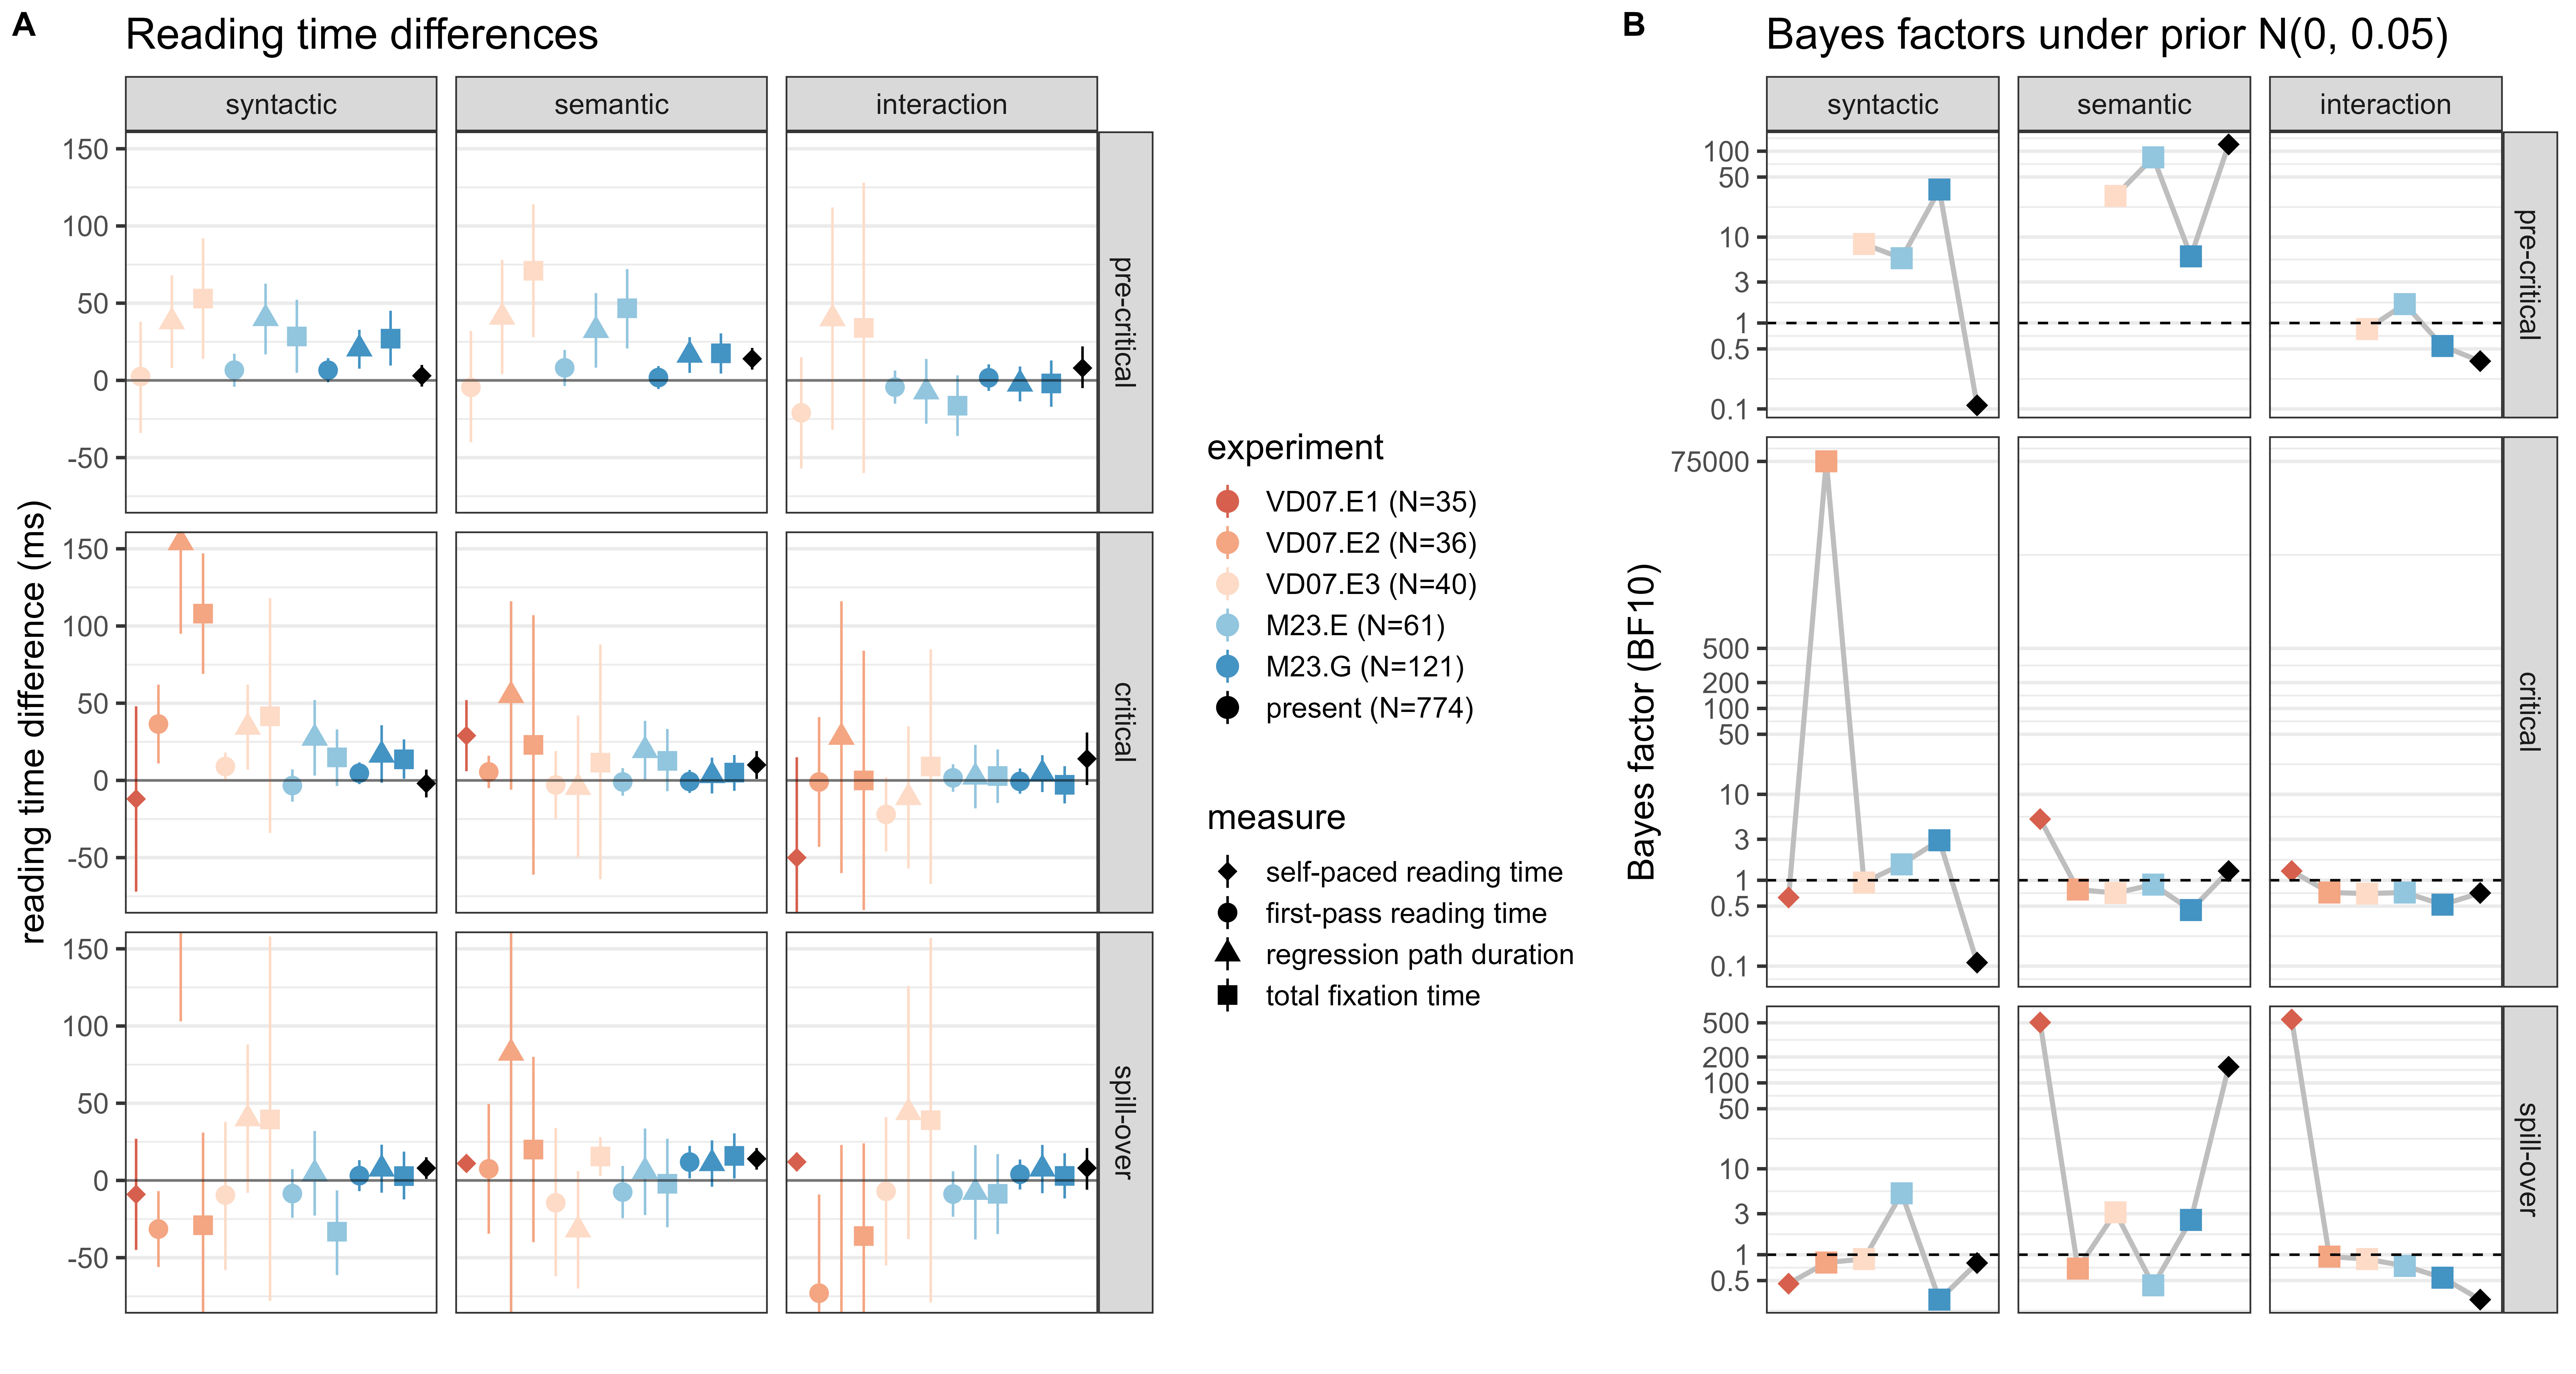
\includegraphics[width=\linewidth]{present_previous_allplots.jpg}
\end{sidewaysfigure}
\clearpage

\subsection*{Comment R1.7}
\begin{quote}
``p. 64: ``Word-by-word presentation is likely to be more demanding on the comprehender's memory, which should make it easier to detect interference effects. So, the differences in methodology do not offer a straightforward
explanation for the lack of syntactic interference in our data compared to the
previous studies."

Actually, I thought here the authors basically provided an explanation of the differences between their findings and the previous findings because of differences in the methodology, even though their last sentence said otherwise. Let me spell out it: since the current methodology (SPR, EEG) is likely more demanding on memory, it is possible that people give up on detailed processing; rather, they do something akin to good-enough processing and do not fully process; consequently, they could still get interference from semantics (since the semantic interference is really simple, it is just lexical semantics and readers don't need to fully parse for that) but they don't correctly parse embedded subjects, hence the syntactic interference is gone. \textbf{The authors in fact come to good-enough processing in Section 7.3, but then it is not linked back to differences between their findings and the other findings (which I think should be, I do think this is a possible explanation).}''
\end{quote}

\subsubsection*{Response to R1.7}
We have added the reviewer's suggested explanation that the employed methods could have especially led to good-enough processing and that this might have contributed to the different findings between studies (see page \pageref{SPR_goodenough}):

\begin{quote}
    \Paste{SPR_goodenough}
\end{quote}

\subsection*{Comment R1.8}
\begin{quote}
``p. 76: \textbf{Chromy should appear like this: ``Chromý" (note the correct diacritics above the ``y")}''
\end{quote}
\subsubsection*{Response to R1.8}
We have corrected the spelling of Jan Chromý's last name.

\section*{Reviewer \#2} 
\subsection*{Comment R2.1}
\begin{quote}
``I appreciate the authors' responses to my previous comments. However, despite the revisions, significant weaknesses remain, rendering in my opinion this study primarily a methodological contribution that adds little value to our understanding of interference effects. Additionally, the authors' strong claims often come through as overstatements that could result in serious misconceptions.
My overall assessment is as follows.

1. Interpretability of the SPR results: The results from the self-paced reading (SPR) task remain unclear. The only observable effect—the semantic interference—emerges well before the critical region of interest (specifically, at the distractor region) and persists without change beyond the critical region. As a result, any effect at the critical region is uninterpretable.

The authors acknowledge the interpretability issue with the SPR results in their response to my comment, and they now include the following statement: ``Given the pre-critical reading time differences, effects in the later regions, i.e., the critical and spill-over regions, cannot be attributed clearly to the stimuli in these regions and sentence processing mechanisms associated with them. Therefore, we refrain from further discussing effects occurring in the later regions." \textbf{However, this comes after more than 10 full pages (pp. 25-37) of discussion on the reaction times (RTs) in the critical and pre-critical regions, which would lead any reader to believe these findings are meaningful. If, as the authors now realize, the effect emerges much earlier, this entire discussion is misleading: the SPR results after the distractor region are simply uninterpretable.}''
\end{quote}

\subsubsection*{Response to R2.1}
We agree with the reviewer that the presentation and discussion of the SPR results was misleading and have revised it accordingly. We have revised Figure 3 to remove the focus on the critical region (see below). At the beginning of the Results section, we now anticipate our interpretation of the results and state that we believe that the distractors led to encoding interference and that the long-lasting effect caused by that confounds the results at later effects. For comparability with previous findings, we then briefly report the later effects. We have revised the Results section in the following way, starting on page \pageref{revised_SPR}: 

\begin{quote}
    \Paste{revised_SPR}
\end{quote}

We do not share the reviewer's interpretation that the effects in the later regions are not meaningful. We use the pre-critical reading times as a proxy to investigate the effect of encoding interference caused by the distractor. To emphasize this we have renamed the former section ``Pre-critical effects" to ``Reading times difference prior to retrieval". We have revised the beginning of the Discussion on page \pageref{prior_to_retrieval} accordingly: 

\begin{quote}
    \Paste{SPR_discussion_revised}
\end{quote}

\setcounter{figure}{2}

\begin{sidewaysfigure}[h]
    \caption{Self-paced reading times with 95\% confidence intervals. Panel A and B show the pooled reading times across the whole sentence; separately for high (A) and low (B) syntactic interference due to differing sentence structure. \textcolor{blue}{Panel C shows the reading times of the sentence focusing on the regions between the distractor and critical verb for all conditions.}}
    \label{fig:whole_sentence}
    \centering
    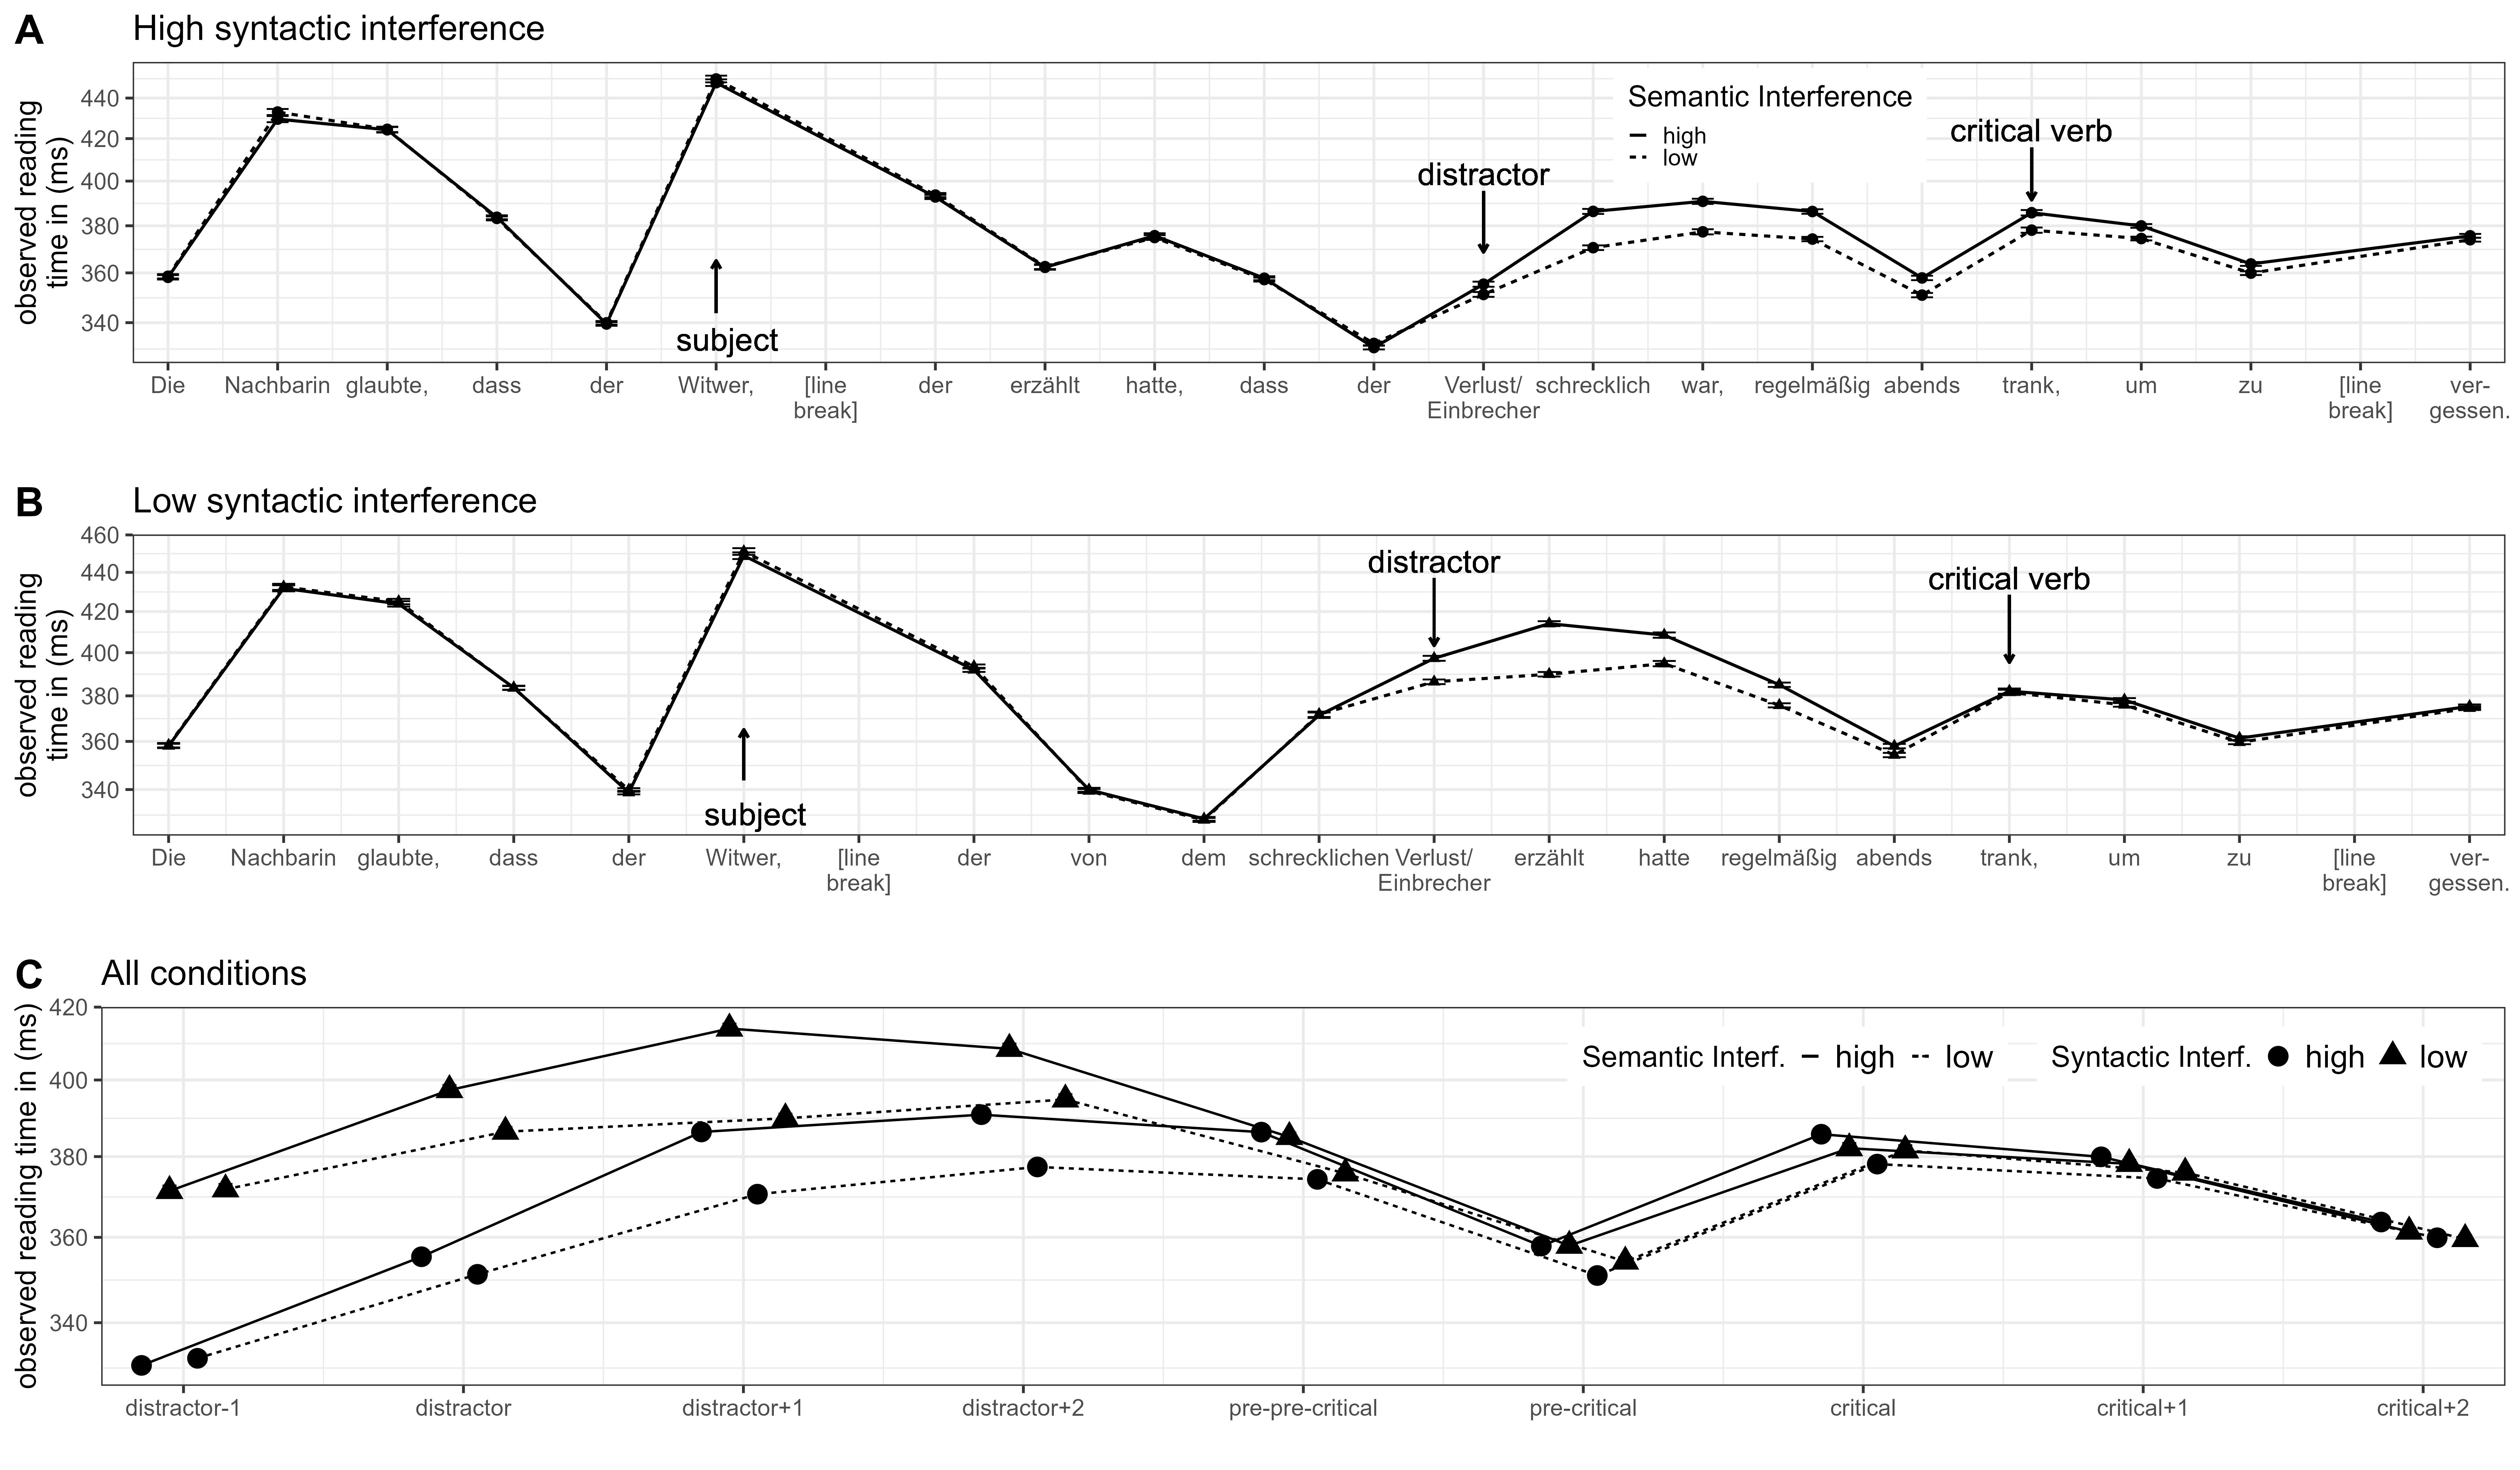
\includegraphics[width=\textwidth]{Pandora_all_wholesentence_pooled_zoom.jpg}
\end{sidewaysfigure}
\clearpage

\subsection*{Comment R2.2}
\begin{quote}
``However, there are also problems with the interpretation of the effect at the distractor region. If the authors want to attribute this effect to encoding interference, then they must argue for the existence of long-lasting encoding effects, as this very same effect persists throughout the entire sentence. Yet, the mechanism behind such enduring encoding effects remains unclear, and the authors do not address this challenge. Feature overlap, a commonly proposed mechanism for encoding interference, seems unlikely. It would suggest that the two elements compete for the same feature throughout the entire sentence, which is not plausible. Activation leveling, another potential mechanism, is also improbable, as it equalizes the activation of competing elements and should result in similar reaction times at some point, which we do not see here. \textbf{What is evident from these findings is that the inanimate distractors are read faster than the animate ones (but the opposite pattern is found in ERPs, see point 3), and this preference creates a reaction time difference that persists until and beyond the critical verb. If the authors wish to interpret this as evidence of encoding interference, they must provide compelling reasons to support the idea that encoding interference can have such a prolonged effect, along a clear mechanism for it}.''
\end{quote}

\subsubsection*{Response to R2.2}
The focus of the present study was to investigate retrieval interference due to syntactic and semantic similarity. The finding that the reading times were primarily affected by encoding interference was unexpected (but see \citeauthor{mertzen}'s (\citeyear{mertzen}) discussion). Given that the present manuscript contains two large-sample experiments and computational modeling (and its substantial length), we think that it is outside the scope of this manuscript to provide an in-depth discussion of a mechanism of encoding interference. Developing a complete treatment of encoding interference would require considerably more computational modeling, which would further increase the length and complexity of this paper. In our opinion, such a model should be developed, but that would need to be a stand-alone article, which would also require more experimental studies to validate and test competing models' predictions. For a recent attempt that we made to try to implement different versions of feature distortion, a phenomenon that is related to encoding interference, see:

Himanshu Yadav, Garrett Smith, Sebastian Reich, and Shravan Vasishth. Number feature distortion modulates cue-based retrieval in reading. Journal of Memory and Language, 129, 2023.

So, in summary, a proper treatment of encoding interference would require a modeling effort at the same scale as was carried out in the above-mentioned paper. Such a modeling effort, although very worthwhile, would take several years' of work and is therefore far beyond the scope of the present work.
 
\subsection*{Comment R2.3}

\begin{quote}
``2. Lack of syntactic interference evidence: No evidence for syntactic interference was found in either task, contradicting two previous studies that tested similar structures (Van Dyke 2007; Mertzen et al. 2023). \textbf{In my previous review, I noted that the syntactic manipulation used was not appropriate and thus unlikely to induce interference effects. Although the authors concede that this might be true, they did not address the logical implications of this acknowledgment, as evidenced by their repeated strong assertions}, such as the one in the abstract: ``Surprisingly, in both experiments, Bayes factor analyses showed evidence against interference due to syntactic cues".
If the syntactic manipulation is irrelevant, then repeatedly concluding that syntactic interference is absent is not only an overstatement but also misleading. All this study allows us to conclude is that when cues that are irrelevant to syntax are manipulated (like [+being a subject of whichever clause at whichever level of embedding], underpowered studies (Van Dyke 2007; Mertzen et al. 2023) may falsely report interference effects. While this is a valid conclusion and a sound methodological critique, it does not significantly advance our theoretical understanding of syntactic interference. Specifically, it fails to demonstrate that when relevant syntactic cues are manipulated, syntactic interference is not attested. Yet, this is the conclusion the authors consistently imply throughout their manuscript, leading to significant misconceptions. As I mentioned in my previous review, beyond the two studies the authors are building on, numerous studies in the literature show that hierarchically intervening elements do generate strong syntactic interference.
It is a fine enterprise to correct inaccurate claims from previously underpowered studies that used irrelevant manipulations; however, this should not not suggest that the findings presented here have a broader significance than they do.''
\end{quote}
\subsubsection*{Response to R2.3}
We agree with the reviewer that our present work does not rule out syntactic interference in general. We have tried to stress throughout the paper that the present study using the present design did not induce considerable syntactic interference. We have revised the abstract and manuscript main body accordingly (see response to E.2). In the general discussion, we have also added the following caveats:

\begin{quote}
    \Paste{gendisccaveat2}
\end{quote}
 
 We feel that the above quote and the other re-statements in the paper (including the abstract) appropriately limit the claims we make in the paper. We never state anywhere in the paper that syntactic interference is generally absent in sentence processing.
  
\subsection*{Comment R2.4}
\begin{quote}
``3. Misalignment of SPR and ERP results: The results from the self-paced reading (SPR) and event-related potential (ERP) methods do not align, with the only observed effect—semantic interference—pointing in opposite directions: inhibitory in SPR but facilitatory in ERP. Specifically, the authors report a reversed effect in the P600 component, showing a reduced P600 in conditions of higher semantic interference. This contradicts typical predictions, where the P600 is usually greater under high interference. The authors interpret this as a facilitatory interference effect (i.e., easier processing with high semantic interference). However, if this were the case, \textbf{we would also expect faster reaction times (RTs) in high semantic interference conditions, while the opposite is observed in the SPR data}.''
\end{quote}

\subsubsection*{Response to R2.4}
The SPR results and the ERP results in the N400 window both show inhibitory interference, i.e., more processing difficulty under high vs.\ low semantic interference, manifesting in longer reading times and a more negative N400. We explain below in our response to R2.5 that the reduced P600 for high interference might be explained by facilitatory interference because under high semantic interference whatever noun was retrieved can be easily integrated. 

In general, SPR results cannot show the same complex results pattern that the ERP results showed because they provide just one measure per region. Additionally, only at the critical (or spill-over) region facilitated integration might be observed and in line with the reviewer's other comments, we do not interpret the reading times of the later regions because these were overshadowed by the reading times differences starting at the distractor.

 
\subsection*{Comment R2.5}
\begin{quote}
``4. Conflicting directions in ERP components: Within the ERP results, the different components also point in opposite directions. The P600 component shows a reversed effect, with a reduced P600 in conditions of high semantic interference. However, the N400 component follows the expected pattern, with stronger activation under high semantic interference. \textbf{It remains unclear how the directionality of these two can be reconciled within the same theoretical framework.}''
\end{quote}

\subsubsection*{Response to R2.5}
 
We have revised our discussion of the ERP results on page \pageref{inhibition_facilitation} to clarify how the seemingly conflicting results can be reconciled (see below). Interference might enhance the N400 amplitude because it makes memory retrieval more difficult and it might reduce the P600 because no matter which noun was retrieved it can be easily integrated with the verb.

\begin{quote}
    \Paste{inhibition_facilitation}
\end{quote}
 
\subsection*{Comment R2.6}
\begin{quote}
``5. Unclear conflicting mechanisms: The authors attribute the SPR results to encoding interference and the ERP results to retrieval interference, leading to a contradictory conclusion. I won't delve further into this point, as the issues raised earlier already highlight more fundamental problems.''
\end{quote}
\subsubsection*{Response to R2.6}
This comment does not call for further action. In section 7.2 ``Encoding and retrieval interference", we discuss that we believe that the difference in presentation rate and whether it was controlled by the participants or not led to different types of interference (encoding vs.\ retrieval).
 
\subsection*{Comment R2.7}
\begin{quote}
``Additional points:

1. Original version: ``By contrast, the syntactic interference effect had only anecdotal evidence under the two narrow priors (Normal-(0, 0.1): BF10 = 2.5, Normal-(0, 0.5): BF10 = 1.2). There was evidence against syntactic interference under wider priors (Normal-(0, 1): BF10 = 0.66, Normal-(0, 5): BF10 = 0.14). What this means is that, in our data, only if we assume a priori that the effect size is relatively small, there is very weak evidence in favor of syntactic interference."

Revised version: ``By contrast, Bayes factors provided either no evidence for or even evidence against syntactic interference in both spatiotemporal windows (BF10 $<$ 1.2). Similarly, Bayes factors provided either no evidence for or even evidence against the interaction in both spatio-temporal windows (BF10 $<$ 1.2)."

\textbf{Did the authors change the analyses? Why what was reported as anecdotal evidence under narrow priors is now reported as no evidence or evidence against?}''
\end{quote}
\subsubsection*{Response to R2.7}
Yes, all analyses were changed in the first round of revision. Firstly, the priors were changed (directional priors in the original version and symmetrical priors in the revised version). Secondly, the method to compute Bayes factors was changed (from bridge sampling to Savage-Dickey, see also our Response to E.3). This resulted in small numerical changes of the results, e.g., BF10 = 2.5 in the original analysis decreased to BF10 = 1.2 in the revised analysis. Furthermore in the original version of the manuscript, we were inconsistent in our description of small BFs, i.e., BF10 = 1.2. Since the first revision and in line with \cite{lee2014bayesian}, we now consistently interpret such small BFs as providing no evidence either way.

 
\subsection*{Comment R2.8}
\begin{quote}
``2. As a side note, on p. 58, the authors conclude that ``the parser searches for a subject that is within the same clause but uses the animacy cue without reference to the clause in which a noun appears." Does this mechanism truly seem plausible to the authors? What would this imply in practice? \textbf{Does it suggest that semantic and syntactic information are entirely encapsulated from each other?} If we were to set aside the issues I raised earlier, this would be one of the paper's central conclusions, yet the authors fail to provide a credible mechanism to support it.''
\end{quote}
\subsubsection*{Response to R2.8}

To clarify the assumed independence of syntactic and semantic processing, we have revised the former section `Relation to other sentence processing accounts', starting on page \pageref{synsem}. We have also renamed the section to `The use of syntactic and semantic information'.

\begin{quote}
    \Paste{synsem}
\end{quote}

 
\subsection*{Comment R2.9}
\begin{quote}
``3. How do the fillers differ from the experimental items? In the example the authors reported there is retrieval at place again:

Experimental: The neighbor believed that the widower, who had told her that the loss was awful, regularly drank in the evenings to forget.\\
Filler: The carpet maker, who came to the workshop early, repaired the especially beautiful old carpet while listening to the news.

The authors state, ``The fillers were less syntactically complex than the experimental items but had at least one embedded clause and generally provided more variety." \textbf{In what way did they provide more variety? In which respects? Both fillers and test items involve retrieval; what is the role of the fillers in this context?}''
\end{quote}
\subsubsection*{Response to R2.9}
The fillers included different types of subordinate clauses and (more) modifiers at different positions within the sentence. By deviating from the rigid structure of the critical items, they provided more variety in regard to the employed sentence structures. To avoid creating an obvious juxtaposition of very complex sentences (critical items) and very simple sentences (fillers), the fillers included long-distance dependencies and at least one subordinate clause. We have revised the description of the fillers in the manuscript on page \pageref{fillers} in the following way:

\begin{quote}
    \Paste{fillers}
\end{quote}
 
\subsection*{Comment R2.10}
\begin{quote}
``4. There are numerous repetitions throughout the paper. A prime example is the paragraph on ``hyp testing using BF" (p. 45), which is repeated almost verbatim in the ``Discussion" section (p. 47). This redundancy occurs several times, making the paper excessively and unnecessarily long. \textbf{The authors should streamline the content to enhance clarity and conciseness.}''
\end{quote}

\subsubsection*{Response to R2.10}
We have removed the repetitions to improve clarity and conciseness (see also Response to E.4).

\section*{Reviewer \#3} 

\begin{quote}
``This is a revision of a paper that I previously reviewed. (I was Reviewer \#3 in the previous round.)

In the previous round of reviews, I was generally happy with the authors' findings. My queries were mostly related to the interpretation and generalizability of those findings. This is a routine issue in psycholinguistic research. A study looks at effects in one very specific (and often complicated) sentence type, and then draws conclusions about very broad notions such as `syntax' and `semantics'.

The authors have offered a thorough (daunting?) response to the reviews. I am more satisfied with some responses than others. But I do not think that this should stand in the way of publication in the JML special issue.

The authors acknowledge the concern about using relational notions such as `subject of the same clause' as a memory retrieval cue. They provide some text that clarifies that they need to implement a clause tracking mechanism. I would prefer it if the text was clearer about the unfeasibility of a `subject of the same clause' feature. But this does not impact their findings.

Another concern that I raised involves the scalability of the notion that semantic interference effects reflect the use of semantic retrieval cues such as [+animate]. At issue is how this extends to finer-grained properties that are routinely responsible for plausibility violations. In my previous review I used the example of ``the teacher drove" vs. ``the little boy drove". It is, of course, clear that teachers are more plausible drivers than young children. This is part of our world knowledge. But it is less plausible that every time the noun `teacher' is encountered the property [+can drive] is activated. The authors' response seems to be that animacy was sufficient for the materials in the current study, and that maybe other finer-grained features ``become activated only when relevant". To my mind, this point removes much of the value of the cue-based retrieval theory. \textbf{Nevertheless, this concern is about the generalizability of the authors' claims, and not about the soundness of their results.}

Finally, and in a similar vein, I raised questions about whether there might be other reasons for the selective interference effects found in this study. Maybe a different mechanism could capture the special status of the subject-of-the-same-clause, or maybe some specific property of the current experimental materials could be responsible for the lack of interference from other subjects. The authors seem skeptical of the first of these, and they seem more sympathetic to the second. \textbf{This is all reasonable enough, and their text conveys some caution. The abstract, on the other hand, is rather more confident.} I am sympathetic to the authors' preferred conclusion. But I am less confident than they are about how well justified it is based on the current findings. This has nothing to do with the quantitative wizardry that the authors display in the paper. It's all about the issue of generalizing from a single sentence configuration (that participants saw in 60\% of trials in the study).''
\end{quote}

\subsubsection*{Response to Reviewer \#3}
We have revised the manuscript (including the abstract) to show more caution regarding the generalizability of our findings (see our response to E.2).


\end{document}  